%  LaTeX support: latex@mdpi.com 

%  For support, please attach all files needed for compiling as well as the log file, and specify your operating system, LaTeX version, and LaTeX editor.

%=================================================================
\documentclass[actuators,article,accept,pdftex,moreauthors]{Definitions/mdpi} 
%\documentclass[preprints,article,submit,pdftex,moreauthors]{Definitions/mdpi} 
% For posting an early version of this manuscript as a preprint, you may use "preprints" as the journal. Changing "submit" to "accept" before posting will remove line numbers.

%--------------------
% Class Options:
%--------------------
%----------
% journal
%----------
% Choose between the following MDPI journals:
% actuators

%---------
% article
%---------
% The default type of manuscript is "article", but can be replaced by: 
% abstract, addendum, article, benchmark, book, bookreview, briefcommunication, briefreport, casereport, changes, clinicopathologicalchallenge, comment, commentary, communication, conceptpaper, conferenceproceedings, correction, conferencereport, creative, datadescriptor, discussion, entry, expressionofconcern, extendedabstract, editorial, essay, erratum, fieldguide, hypothesis, interestingimages, letter, meetingreport, monograph, newbookreceived, obituary, opinion, proceedingpaper, projectreport, reply, retraction, review, perspective, protocol, shortnote, studyprotocol, supfile, systematicreview, technicalnote, viewpoint, guidelines, registeredreport, tutorial,  giantsinurology, urologyaroundtheworld
% supfile = supplementary materials

%----------
% submit
%----------
% The class option "submit" will be changed to "accept" by the Editorial Office when the paper is accepted. This will only make changes to the frontpage (e.g., the logo of the journal will get visible), the headings, and the copyright information. Also, line numbering will be removed. Journal info and pagination for accepted papers will also be assigned by the Editorial Office.

%---------
% pdftex
%---------
% The option pdftex is for use with pdfLaTeX. Remove "pdftex" for (1) compiling with LaTeX & dvi2pdf (if eps figures are used) or for (2) compiling with XeLaTeX.

%=================================================================
% MDPI internal commands - do not modify
\firstpage{1} 
\makeatletter 
\setcounter{page}{\@firstpage} 
\makeatother
\pubvolume{1}
\issuenum{1}
\articlenumber{0}
\pubyear{2026}
\copyrightyear{2026}
\externaleditor{Firstname Lastname} % More than 1 editor, please add `` and '' before the last editor name
\datereceived{2 March 2026} 
\daterevised{14 April 2026} % Comment out if no revised date
\dateaccepted{17 April 2026} 
\datepublished{ } 
%\datecorrected{} % For corrected papers: "Corrected: XXX" date in the original paper.
%\dateretracted{} % For retracted papers: "Retracted: XXX" date in the original paper.
%\doinum{} % Used for some special journals, like molbank
%\pdfoutput=1 % Uncommented for upload to arXiv.org
%\CorrStatement{yes}  % For updates
%\longauthorlist{yes} % For many authors that exceed the left citation part
%\IsAssociation{yes} % For association journals

%=================================================================
% Add packages and commands here. The following packages are loaded in our class file: fontenc, inputenc, calc, indentfirst, fancyhdr, graphicx, epstopdf, lastpage, ifthen, float, amsmath, amssymb, lineno, setspace, enumitem, mathpazo, booktabs, titlesec, etoolbox, tabto, xcolor, colortbl, soul, multirow, microtype, tikz, totcount, changepage, attrib, upgreek, array, tabularx, pbox, ragged2e, tocloft, marginnote, marginfix, enotez, amsthm, natbib, hyperref, cleveref, scrextend, url, geometry, newfloat, caption, draftwatermark, seqsplit
% cleveref: load \crefname definitions after \begin{document}
\usepackage{siunitx}
\let\DeclareUSUnit\DeclareSIUnit
\let\US\SI
\DeclareUSUnit\inch{in}
\DeclareUSUnit\inch{in}
\providecommand{\abs}[1]{\lvert#1\rvert}
\providecommand{\norm}[1]{\lVert#1\rVert}
\usepackage{graphicx}
\usepackage{caption}
\usepackage{multicol}
\usepackage{array}



%=================================================================
% Please use the following mathematics environments: Theorem, Lemma, Corollary, Proposition, Characterization, Property, Problem, Example, ExamplesandDefinitions, Hypothesis, Remark, Definition, Notation, Assumption
%% For proofs, please use the proof environment (the amsthm package is loaded by the MDPI class).

%=================================================================
% Full title of the paper (Capitalized)
\Title{Isometric Force Characterization of Braided Pneumatic Actuators}

% Author Orchid ID: enter ID or remove command
\newcommand{\orcidauthorA}{0000-0003-3789-7205} % Add \orcidA{} behind the author's name
\newcommand{\orcidauthorB}{0009-0008-9985-0676} % Add \orcidB{} behind the author's name
\newcommand{\orcidauthorC}{0000-0002-3820-4821} % Add \orcidC{} behind the author's name

% Authors, for the paper (add full first names)
\Author{\hl{Ben Bolen *\orcidA{},} %MDPI: 1. Please carefully check the accuracy of names and affiliations.  2. Only one affiliation of the text, we removed affiliation numbers, please confirm. 3. The corresponding author is different from the ones submitted online at susy.mdpi.com. Please confirm which one is correct. 4. Please confirm if keep orcid numbers in text.
 Mohammad Elzein \orcidB{}, Lawrence Pang and \hl{Alexander Hunt \orcidC{}} %MDPI: The name is different from the ones submitted online at susy.mdpi.com. Please confirm which one is correct.
}

%\longauthorlist{yes}

% MDPI internal command: Authors, for metadata in PDF
\AuthorNames{Ben Bolen, Mohammad Elzein, Lawrence Pang and Alexander Hunt}

% Affiliations / Addresses (Add [1] after \address if there is only one affiliation.)
\address[1]{Department of Mechanical and Materials Engineering, Portland State University, Portland, \hl{OR,} %MDPI: Please add the postal code (or ZIP code in the U.S.). If a postal code is not available, a Post Office Box number can be added instead.
 USA; \hl{melzein@pdx.edu (M.E.); lawrence\_91096@hotmail.com (L.P.); ajh26@pdx.edu (A.H.)} %MDPI: We added these email addresses here according to those submitted online at susy.mdpi.com. Please confirm.
}


% Contact information of the corresponding author
\corres{\hangafter=1 \hangindent=1.05em \hspace{-0.82em} Correspondence: bbolen83@gmail.com}

% Current address and/or shared authorship
%\firstnote{Current address: Affiliation.}  
% Current address should not be the same as any items in the Affiliation section.

%\secondnote{These authors contributed equally to this work.}
% The commands \thirdnote{} till \eighthnote{} are available for further notes.

%\simplesumm{} % Simple summary

%\conference{} % An extended version of a conference paper

% Abstract (Do not insert blank lines, i.e. \\) 
\abstract{Artificial muscles such as braided pneumatic actuators (BPAs) offer many advantages for robotic systems, including high durability and strength-to-weight ratios. However, their use in robotic systems is still extremely limited, in part due to their poor force, length, and pressure characterization. In this work, a test setup is created to compare force produced by Festo fluidic BPAs with leading models. Our analysis of the data has resulted in (1) the development of new equations to calculate force as functions of pressure and contraction for Festo BPAs with uninflated diameters of \qtylist{10;20}{\mm}, and (2) a novel equation for the maximum force in \qtylist{10;20}{\mm} diameter Festo BPAs as a function of their resting length. This will lead to faster design processes and the development of new systems such as biomimetic robots that are able to more accurately reproduce the range of motion and isometric torque profiles that exist in the animals they are mimicking.}

% Keywords
\keyword{BPA; \highlighting{biomimetic;} %MDPI: We revised keywords format in the part, please check and confirm in whole text.
 function fit; PAM; artificial muscle; isometric force} 

% The fields PACS, MSC, and JEL may be left empty or commented out if not applicable
%\PACS{J0101}
%\MSC{}
%\JEL{}

%%%%%%%%%%%%%%%%%%%%%%%%%%%%%%%%%%%%%%%%%%
% Different journals have different requirements. Please check the specific journal guidelines in the "Instructions for Authors" on the journal's official website.
\addhighlights{yes}
\renewcommand{\addhighlights}{%
%
%\noindent The goal is to increase the discoverability and readability of the article via search engines and other scholars. Highlights should not be a copy of the abstract, but a simple text allowing the reader to quickly and simplified find out what the article is about and what can be cited from it. Each of these parts should be devoted up to 2~bullet points.\vspace{3pt}\\
%\textbf{What are the main findings?}
\begin{itemize}[labelsep=2.5mm,topsep=-3pt]
\item \hl{Braided} %MDPI: The journal seems to be not allowed highlights, please confirm if the part is necessary, if is, it is recommended to use the Q&A format, like below:
%\textbf{What are the main findings?}
% \begin{itemize}[labelsep=2.5mm,topsep=-3pt]
% \item First bullet.
% \item Second bullet.
% \end{itemize}\vspace{3pt}
%\textbf{What is the implication of the main finding?}
% \begin{itemize}[labelsep=2.5mm,topsep=-3pt]
% \item First bullet.
% \item Second bullet.
% \end{itemize}
 Pneumatic Actuator maximum isometric force is a function of resting length.
\item Force curves are normalized with pressure and maximum contraction.
\item A high-fidelity predictive force model is developed using few coefficients.
\end{itemize}
}

%%%%%%%%%%%%%%%%%%%%%%%%%%%%%%%%%%%%%%%%%%
\begin{document}




\section{Introduction}\label{introduction}
Biomimetic robots provide a platform for investigating how mechanical structure and control interact to generate movement, offering complementary insights to simulation-based studies \citep{andrews_general_1985, millard_flexing_2013, arnold_model_2010}. Musculoskeletal humanoids and limb systems driven by tendon-like actuators have been shown to support biologically meaningful experiments on motion generation, internal force transmission, and neural control hypotheses \citep{asano_design_2017, asano_musculoskeletal_2019, hitzmann_anthropomorphic_2018, liu_robotic_2018, chen_realizing_2019}. This dual perspective of using robots to learn about biology and using biology to design more adaptive robots has been emphasized in both biomimetic robotics and biomechanics \citep{ijspeert_amphibious_2020, asano_design_2017}.

A wide range of actuation technologies have been explored in robotics, including electric motors, hydraulic systems, smart-material actuators, and artificial muscles \citep{he_mechanism_2020, liang_comparative_2020}. Electric motors are widely used due to their controllability and maturity, but are limited by thermal constraints, gearing requirements, and reduced compliance compared to muscle-like actuators \citep{veale_towards_2016, suzumori_trends_2018}. Hydraulic actuators offer exceptionally high power density and have enabled highly dynamic legged systems, but they remain relatively heavy, less efficient than biological muscle, and require a dedicated fluid infrastructure \citep{suzumori_trends_2018}. Dielectric elastomer actuators (DEAs), a class of electronic electroactive polymers, demonstrate high specific work and good bandwidth in comparative studies \citep{liang_comparative_2020}. However, they are limited by the need for kilovolt-range driving voltages \citep{madden_artificial_2004}, electromechanical instability, and the requirement for compliant electrodes \citep{liang_comparative_2020}. In contrast, McKibben-style braided pneumatic actuators (BPAs) combine low mass, high force-to-weight ratio, and intrinsic compliance with a force–length curve that qualitatively resembles that of skeletal muscle \citep{liang_comparative_2020, hunt_modeling_2017}. BPAs have been used in quadrupedal robots \citep{aschenbeck_design_2006, hunt_modeling_2017}, musculoskeletal humanoids \citep{asano_design_2017, hitzmann_anthropomorphic_2018}, and dexterous manipulation systems \citep{chen_realizing_2019}, demonstrating their ability to support biologically motivated investigations and improve robot adaptability in unstructured environments.

Despite these advantages, BPAs exhibit several important differences from biological muscle. First, BPA maximum tensile force occurs at resting (i.e., uninflated) \hl{length} %MDPI: Please carefully check variable formatting (italic, bold, subscript, uppercase, etc.) throughout the manuscript to ensure the formatting is consistent and revise if needed, and please confirm if there is duplicated equations, if yes, please confirm if they are right.
 ($l_{rest}$) rather than at an optimal fiber length \citep{liang_comparative_2020}. Second, their maximum contraction ratio is substantially lower than that of human muscle, presenting challenges for achieving biomimetic joint ranges of motion \citep{hunt_modeling_2017, sarosi_comparative_2017, liang_comparative_2020}. Third, BPAs have a highly nonlinear dependence on internal pressure ($P$), contraction ($\epsilon$), and loading state \citep{hunt_modeling_2017, martens_modeling_2017}, which complicates control and motivates high-fidelity force–length–pressure modeling.

To address these challenges, numerous researchers have proposed static and dynamic models for BPAs. \citet{sarosi_comparative_2017} compared geometric and empirical models for uninflated diameters ($\phi$) \qty{10}{\mm} and \qty{20}{\mm} actuators and highlighted limitations when $l_{rest}$ varies. \citet{martens_modeling_2017} introduced a physically motivated static model for the \hl{Festo} %MDPI: Please state which version of the software was used.
 DMSP series and demonstrated accurate predictions at specific $l_{rest}$. Festo provides a manufacturer tool for predicting force as a function of pressure and contraction \citep{festo_2026, lang_robert_musclesim_2005}, but experimental comparisons indicate that it does not adequately account for variation in $l_{rest}$ or actuator-specific contraction limits. \citet{hunt_modeling_2017} developed a more generalizable empirical model for $\phi$\qty{10}{\mm} Festo BPAs that incorporates differences between eccentric and concentric loading states and accounts for the maximum achievable contraction ($\epsilon_{max}$) at high pressures. Comparisons with experimental data indicate that none of the existing models effectively take into account differences in maximum force due to initial \mbox{actuator length.}

The present work develops an improved force–pressure–length model for both $\phi$\qty{10}{\mm} and $\phi$\qty{20}{\mm} Festo BPAs. We collected extensive force data for a wide range of resting lengths, contraction ratios, and internal pressures. These data were first used to find maximum force as a function of resting length. Then we normalized the data to formulate normalized force ($F^*$) as a function of relative strain ($\epsilon^*$) and relative pressure ($P^*$). The resulting model provides improved predictive accuracy for isometric BPA force, supporting the design and control of biomimetic robotic systems that rely on BPAs.



\section{Background}

\hl{Previous} %MDPI: This is a reminder:1. The companies/manufacturers of chemicals & reagents, devices, instruments, commercial cell lines/samples/materials should be indicated together with their city (state/province abbreviation is required for USA and Canada) and country in their first appearance. Please add necessary information for those items in text. For all the soft-ware used, please add the information of them.2. For all the software used, Please state the version number of the software. If it is not applicable, the related website or proof should be provided. Please review the full text and make sure each software has a version number or website.
 studies have generated empirical models of the force--length--pressure relationship of BPAs. \citet{sarosi_comparative_2017} discuss several high-fidelity BPA force models. They present a static force model with a 21 coefficient polynomial function for a \hl{Festo MAS-20-200N} %MDPI: Please state the name of the manufacturer, city, and country from where the equipment was sourced. The following highlights are the same.
 (i.e., $\phi$\qty{20}{\mm}, $l_{rest}=\qty{200}{\mm}$) with an impressive $\text{R}^2=0.9994$. They also present Sárosi's static force model for a \hl{Festo DMSP-20-400N-RM-RM} (i.e., \highlighting{$\phi$\qty{20}{\mm},} %MDPI: Please confirm if needs to add a space between ϕ and numbers, please check and confirm all in whole text.
 $l_{rest}=\qty{400}{\mm}$), with six coefficients and a $\text{R}^2=0.9995$. Martins and Boblan present an even more accurate model, in terms of absolute error, using five coefficients for a \hl{DMSP-10-250} (i.e., $\phi$\qty{10}{\mm}, $l_{rest}=\qty{250}{\mm}$) and a \hl{DMSP-20-300} (i.e., $\phi$\qty{20}{\mm}, $l_{rest}=\qty{300}{\mm}$) \citep{martens_modeling_2017}.  However, our work, as presented below, demonstrates that different resting lengths produce different force--length curves, preventing the use of these models for designing systems with different resting lengths.

\citet{hunt_modeling_2017} looked at six resting lengths of $\phi$\qty{10}{\mm} Festo BPAs, accounting for differences in maximum contractile percentages, and elucidating the force--length--pressure relationship. In particular, for a given contraction percent and force $F$ (in Newtons), the scalar pressure $P$ (in kPa) required to produce this force for a $\phi$\qty{10}{\mm} Festo artificial muscle can be determined by solving the equation:
\begin{adjustwidth}{-\extralength}{0cm}
\begin{equation}
P = \qty{254}{\kPa} + F \cdot \qty{1.23}{\kPa\per\newton} + S \cdot \qty{15.6}{\kPa} + \qty{192}{\kPa} \cdot \tan\,\left( 2.03 \left( \frac{\epsilon}{\epsilon_{\max} - F \cdot \qty{0.331e-3}{\per\newton}} - 0.46 \right) \right)
\end{equation} \label{eq:BPAFit}
\end{adjustwidth}
where $S$ is the artificial muscle hysteresis factor such that $S=1$ indicates the muscle is shortening, $S=-1$ indicates it is lengthening, and $S=0$ under static conditions. An important note for Equation~(\ref{eq:BPAFit}) is that the coefficients have been updated with the correct values as the values reported in \cite{hunt_modeling_2017} contained typographical errors. The amount of contraction, ${\epsilon}$, is calculated as
\begin{equation}
    \epsilon = \frac{(l_{rest}-l)}{l_{rest}} \label{eq:strain}
\end{equation}
where ${\epsilon_{620}}$ is the amount of contraction in a BPA without external load when inflated at $\qty{620}{\kPa}$ (90 psi), similarly calculated as 
\begin{equation}
    \epsilon_{620} = \frac{(l_{rest}-l_{620})}{l_{rest}} \label{eq:max_strain}
\end{equation}
where $l_{620}$ is defined as the muscle length measured at 620 kPa. 
Equation~(\ref{eq:BPAFit}) was used to create a lookup table for actuator force, $F$, for a given amount of pressure, $P$, and relative contraction, $\epsilon^*$, defined as
\begin{equation}
    \epsilon^* = \frac{\epsilon}{\epsilon_{620}} \label{eq:rel_strain}
\end{equation}
using the results from Equations~(\ref{eq:strain}) and (\ref{eq:max_strain}).

However, this model was taken with low external forces ($\leq$24 lbs), and it is unclear how well this model captures actuator behavior at higher forces, so we compare this model with data collected in this work.

%%%%%%%%%%%%%%%%%%%%%%%%%%%%%%%%%%%%%%%%%%
\section{Materials and Methods}

\subsection{Overview}

To measure artificial muscle force as a function of length and pressure, we built a test jig from extruded alumnium and 3D printed parts. Festo BPAs with \qtylist{10;20}{\mm} diameter were tested with various resting lengths and different amounts of contraction. These data are used to develop an improved model that more accurately predicts maximum muscle force based on $l_{rest}$, current muscle length $l_{m}$, and pressure $P$. The results are compared with existing models and the new data are used to create an updated model. 

\subsection{BPA Force Characterization Experiment}
A test jig was made of 80/20\textsuperscript{{\textregistered}} brand 1515 series extruded aluminum (Figure~\ref{fig:testJig}). Artificial muscles were placed vertically in the jig one at a time. The upper end was attached to an S-shaped load cell. The lower end was attached to an adjustable crossmember that was used to change the actuator length $l_{m}$. Compressed air was supplied through the building at \qty{620}{\kPa} and measured with a \hl{Freescale MPX5700 pressure sensor}. 

The inner distance between the hose clamps on each BPA was measured to determine the muscle's resting length ($l_{rest}$). This is how \citet{festo_2026} defines $l_{rest}$, although in \citet{hunt_modeling_2017} it was measured to also include end cap length. We then inflated each BPA to $P_{620}=\qty{620}{kPa}$, with one end allowed to move freely in the axial Degree of Freedom (DoF), and measured the length $l_{620}$ to calculate maximum contraction at \qty{620}{\kPa} using Equation~(\ref{eq:max_strain}). The distance between the crossmembers was then controlled to obtain different amounts of contraction, the muscles were inflated to various pressures, and the contractile force was recorded at the pressure--contraction pairs. This was done for $\phi$\qty{10}{\mm} BPA resting lengths ($l_{rest}$) of \SIrange[range-phrase=--]{112}{518}{\mm}. For $\phi$\qty{20}{\mm} BPAs, resting lengths ($l_{rest}$) of \SIrange[range-phrase=--]{300}{509}{\mm} were used.

%The BPAs were then deflated, placed vertically in the test jig made out of 80/20 1515 series extruded aluminum pieces and fixed between two crossmembers.  The force sensor was placed between the upper crossmember and the BPA. $\phi$\qty{10}{\mm} BPAs with $l_{rest}$ of \qtylist{120;220;260;281;281}{\mm} had a lot of $P$ variation, with only 4--5 different values of $\epsilon^*$ per BPA. Conversely, BPAs with $l_{rest}$ of \qtylist{112;415;455;490;518}{\mm} had many different values of $\epsilon^*$ recorded, but all values were taken at or near $P_{max}$.

\begin{figure}[H]%[htbp]
   % \begin{center}
   \hspace{-11mm} 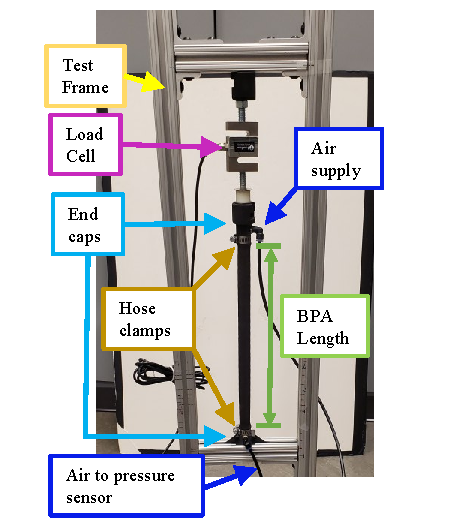
\includegraphics[width=0.75\textwidth]{01_testJigs1.pdf}
 %   \end{center}
    \caption{\hl{A} %MDPI: 1. Please confirm whether the overlapping/incomplete content in this figure affects scientific understanding and if it does, please revise it. 2. Please note that the size of figures and tables, the position of figures and tables will be adjusted appropriately may occur during the production stage to reduce the page blank.
 picture of a BPA in the isometric force test stand with components labeled.}\label{fig:testJig}
\end{figure}

%%%%%%%%%%%%%%%%%%%%%%%%%%%%%%%%%%%%%%%%%%
\section{Results}

\subsection{Maximum Force at 620 kPa}

Data of the maximum force from BPA characterization tests of the \qty{10}{\mm} and \qty{20}{\mm} diameters at \qty{620}{\kPa} show a dependency on resting length (Figure~\ref{fig:Fmax_fit}). This is a previously unreported characteristic of these artificial muscles. Detailed analysis of the Festo \mbox{tool \citep{festo_2026}} does in fact predict a change in maximum force with the resting length; however, the Festo tool predicts increased force with shorter lengths, while our collected data indicate decreasing force with shorter lengths. The data show a force response resembling an $\arctan$ curve along the $l_{rest}$ dimension. Using the Nonlinear Least Squares method and a Least Absolute Residual robustness, we fit an arctan curve to the data to get the maximum force at \qty{620}{\kPa} given a resting length as:
\begin{align}
    F_{620_{10}} &= \qty{303.5}{\N}\cdot \arctan{( \qty{19.03}{\per\metre} \cdot (l_{rest}-0.0075))}  \label{eq:Fmax10} \\[10pt]
    F_{620_{20}} &= \qty{922.4}{\N} \cdot \arctan{(\qty{15.37}{\per\m} \cdot (l_{rest}-0.013))} \label{eq:Fmax20}
\end{align}

\noindent
\hl{The} %MDPI: Please confirm if the noindent of paragraph is necessary in whole text. Please check and confirm all.
 length is offset by \qty{0.0075}{\m} and \qty{0.013}{\m} because solid modeling showed that the end caps contact each other at these lengths. At these lengths, the actuator would not be able to contract to produce force.


\begin{figure}[H]%[tbp]
%\begin{adjustwidth}{-\extralength}{0cm}
%\centering
\subfloat[\centering]{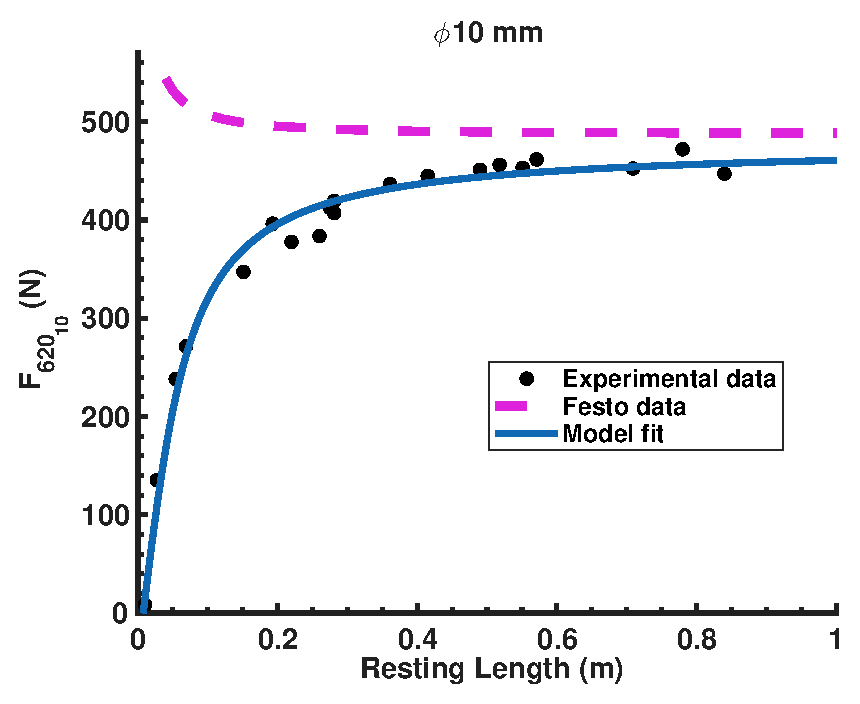
\includegraphics[width=13.8cm]{02a_MaxForce10.eps}}\\
\subfloat[\centering]{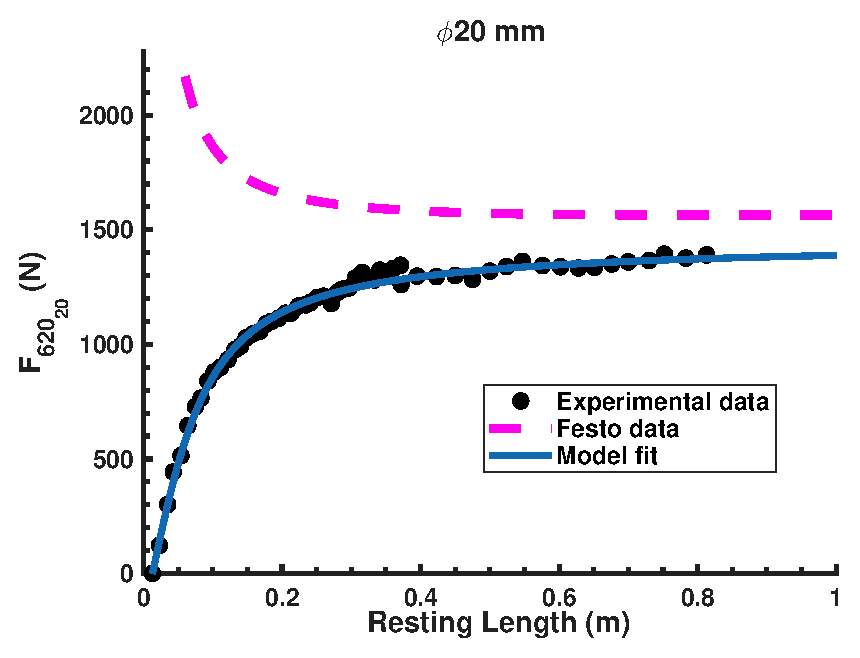
\includegraphics[width=13.8cm]{02b_MaxForce20.eps}}
%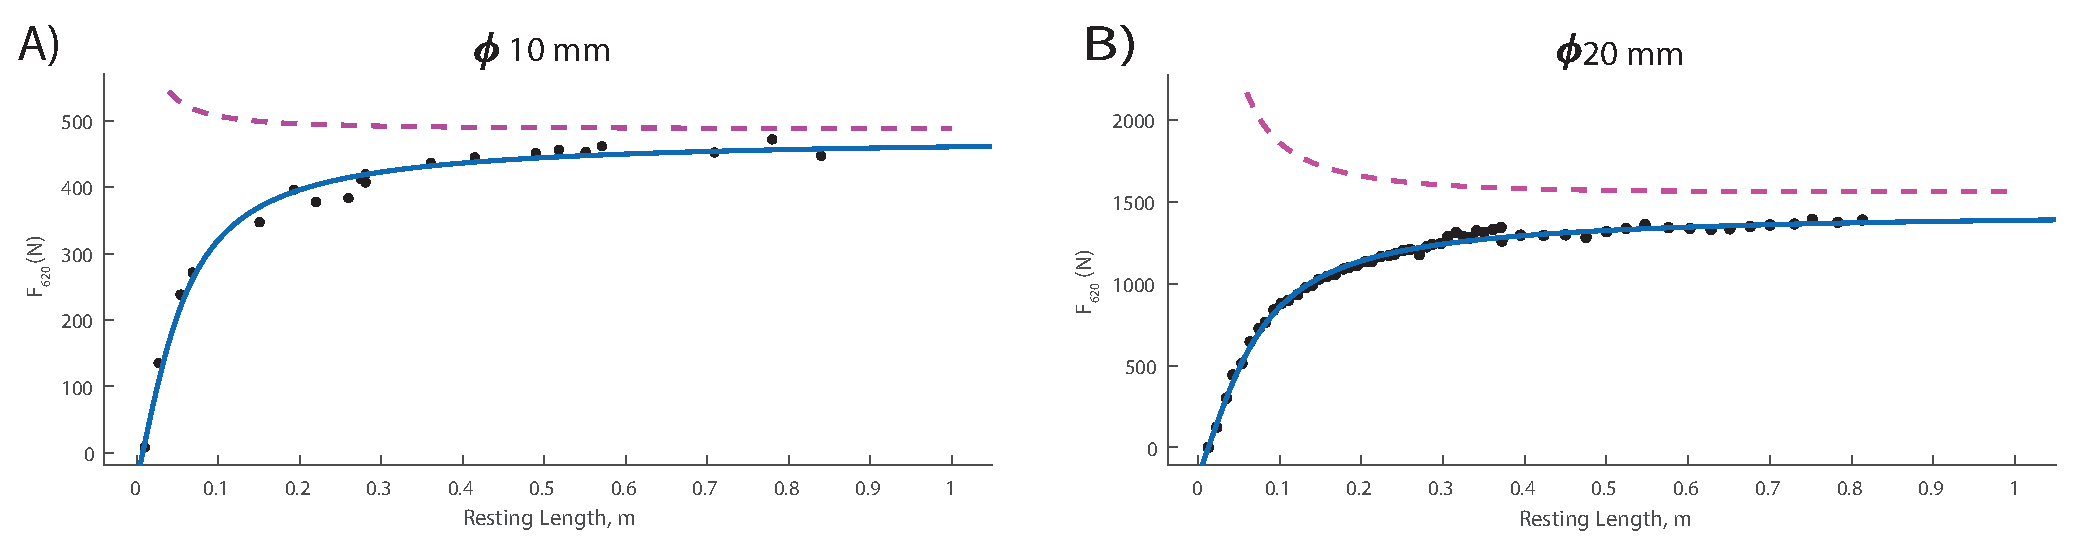
\includegraphics[width=1\textwidth]{02_Fmax_fit.eps}
%\end{adjustwidth}
\caption{Results for finding the relationship between $F_{620}$ and $l_{rest}$. (\textbf{a}) $F_{620_{10}}$ as a function of $l_{rest}$, at $P_{620}$. Dashed line is the $F_{620_{10}}$ data from Festo. Solid line is the fit from Equation (\ref{eq:Fmax10}). (\textbf{b}) $F_{620_{20}}$ as a function of $l_{rest}$ at $P_{620}$. Dashed line is $F_{620_{20}}$ data from Festo. Solid line is the fit from Equation (\ref{eq:Fmax20}).}\label{fig:Fmax_fit}
\end{figure}


%Data from BPA characterization tests of the \qty{10}{\mm} muscles resulted in force-pressure pairings for different muscle resting lengths ($l_{rest}$) Figure~\ref{fig:Fmax_fit}\textbf{A}. Analysis of the data showed that the maximum isometric force ($F_{max}$) produced by the actuator at its resting length is a function of resting length $l_{rest}$ (Figure~\ref{fig:Fmax_fit}B), a previously unreported characteristic of these artificial muscles. The data show a force response resembling an $\arctan$ curve along the $l_{rest}$ dimension and with a more linear response with changes in pressure. Using the Nonlinear Least Squares method and a Least Absolute Residual robustness, we fit an arctan curve to the data at to get the maximum force given a resting length and pressure as:

\subsection{Force as a Function of Pressure and Resting Length}

Data from BPA characterization tests of the \qty{10}{\mm} muscles resulted in force--pressure pairings for different muscle resting lengths ($l_{rest}$) (Figure~\ref{fig:F-P_contraction}\hl{a}%MDPI: We revised label number format to keep consistent with image, please confirm. Same as below.
). Similar to the maximum force data, these data show a force response resembling an $\arctan$ curve along the $l_{rest}$ dimension  with a more linear response to changes in pressure. Using the Nonlinear Least Squares method and a Least Absolute Residual robustness, we fit an arctan curve to the data to get the maximum force given a resting length and pressure as:
\begin{equation}
    F_{max}(l_{rest},P) = a_1 \cdot P \cdot \arctan{(a_2 \cdot P \cdot (l_{rest}-0.0075))} \label{eq:Fmax_3D}
\end{equation}
where $a_1 = \qty{0.4895}{\N\per\kPa}$  and $a_2=\qty{0.03068}{\per\kPa\per\m}$ for the \qty{10}{\mm} actuator, and \mbox{$a_1 = \qty{1.49}{\N\per\kPa}$,} $a_2=\qty{0.0248}{\per\kPa\per\m}$ for the \qty{20}{\mm} actuator. Goodness-of-fit measures are given in Table~\ref{tab:Fmax}. 



\begin{table}[H]
\caption{\hl{Maximum} %MDPI: 1. We removed verticle lines in table, please confirm. 2. Please confirm if the center, left and right alignments necessary in table. 3. We put table not in landscape, please confirm. 4. We inserted it after where it is first mentioned in the text, please check and confirm.
 force equation coefficient values with confidence intervals (CI) and goodness-of-fit measures. Equation~(\ref{eq:Fmax_3D}) is compared to data taken at \qty{620}{\kPa} . Equations~(\ref{eq:Fmax10}) and (\ref{eq:Fmax20}) are compared against maximum force from using the Festo tool. It was not necessary to fit an adjusted $\text{R}^2$ in \mbox{these cases.}} 
\label{tab:Fmax}
\small
\begin{adjustwidth}{-\extralength}{0cm}
%\centering %% If there is a figure in wide page, please release command \centering
\begin{tabularx}{\fulllength}{cllllrclr}
\toprule
\multirow{2}{*}{\textbf{Equation}} &
  \multirow{2.1}{*}{\textbf{Coefficient}} &
  \multirow{2.2}{*}{\textbf{CI (95\%)}} &
  \multicolumn{3}{c}{\textbf{Our Model}} &
  \multicolumn{3}{c}{\textbf{Festo Tool}} \\  
 &
   &
   &
  \multicolumn{1}{l}{\textbf{Adj. $\text{R}^2$}} &
  \multicolumn{1}{l}{\textbf{RMSE}} &
  \textbf{Max. Error} &
  \multicolumn{1}{l}{\textbf{Adj. $\text{R}^2$}} &
  \multicolumn{1}{l}{\textbf{RMSE}} &
  \textbf{Max. Error} \\ \midrule 
\multirow{2}{*}{\eqref{eq:Fmax_3D}} &
  $a_1 =   \qty{0.4895}{\N\per\kPa}$ &
  (0.4822, 0.4968) &
  \multicolumn{1}{l}{\multirow{2}{*}{0.9945}} &
  \multicolumn{1}{l}{\multirow{2}{*}{11.61 N}} &
  \multirow{2}{*}{55.3 N} &
  \multicolumn{1}{l}{\multirow{2}{*}{0.9854}} &
  \multicolumn{1}{l}{\multirow{2}{*}{14.7 N}} &
  \multirow{2}{*}{30.9 N} \\ 
 &
  $a_2 =   \qty{0.03068}{\per\kPa\per\m}$ &
  (0.0282, 0.03317) &
  \multicolumn{1}{l}{} &
  \multicolumn{1}{l}{} &
   &
  \multicolumn{1}{l}{} &
  \multicolumn{1}{l}{} &
   \\ \midrule
\multirow{2}{*}{\eqref{eq:Fmax10}} &
  $b_1   =\qty{303.5}{\N}$ &
  (300, 308) &
  \multicolumn{1}{l}{\multirow{2}{*}{0.9854}} &
  \multicolumn{1}{l}{\multirow{2}{*}{14.72 N}} &
  \multirow{2}{*}{30.9 N} &
  \multicolumn{1}{c}{\multirow{2}{*}{\hl{--} %MDPI: Please confirm if it needs an explanation.
}} &
  \multicolumn{1}{l}{\multirow{2}{*}{189.9 N}} &
  \multirow{2}{*}{375.6 N} \\ 
 &
  $b_2 =   \qty{19.03}{\per\m}$ &
  (17.48, 20.57) &
  \multicolumn{1}{l}{} &
  \multicolumn{1}{l}{} &
   &
  \multicolumn{1}{l}{} &
  \multicolumn{1}{l}{} &
   \\ \midrule
\multirow{2}{*}{\eqref{eq:Fmax20}} &
  $b_1 =   \qty{922.4}{\N}$ &
  (914.2, 930.7) &
  \multicolumn{1}{l}{\multirow{2}{*}{0.9945}} &
  \multicolumn{1}{l}{\multirow{2}{*}{23.83 N}} &
  \multirow{2}{*}{62.1 N} &
  \multicolumn{1}{c}{\multirow{2}{*}{--}} &
  \multicolumn{1}{l}{\multirow{2}{*}{668.4 N}} &
  \multirow{2}{*}{1590.1 N} \\ 
 &
  $b_2=\qty{15.37}{\per\m}$ &
  (14.75, 15.98) &
  \multicolumn{1}{l}{} &
  \multicolumn{1}{l}{} &
   &
  \multicolumn{1}{l}{} &
  \multicolumn{1}{l}{} &
   \\ \bottomrule
\end{tabularx}
\end{adjustwidth}
\end{table}






\subsection{Maximum Contraction at \qty{620}{\kPa}}

Figure~\ref{fig:F-P_contraction}\hl{b} shows an attempt at a linear fit for maximum contraction at \qty{620}{\kPa} ($\epsilon_{620}$) as a function of resting length ($l_{rest})$. Error bars have been included to show the effect of $\pm$\qty{1}{\mm} accuracy with measurements of $l_{rest}$ and $l_{620}$. There was a large amount of variance in the data, with the linear fit giving an adjusted $\text{R}^2=0.4124$ and an $\text{RMSE}=0.0083$. Since there is no direct, predicable relationship between maximum contraction and $l_{rest}$, this value should be recorded in each muscle used on a robot to best predict the force it may produce at different pressures and contraction. 


\subsection{Force as a Function of Pressure and Contraction}

In addition to being a function of the pressure and resting length, the force produced by the actuator is also a function of the amount of actuator contraction, with less force being applied as the actuator contracts. 
To build this model, the collected data of force, pressure, and contraction are normalized by dividing by $F_{620}$, $P_{620}$, and $\epsilon_{620}$, respectively. This had the effect of compressing the data into a 3D surface ranging from 0 to 1 on all axes. Normalized data are compared with pressure isoclines of force predicted by the Festo tool divided by the maximum force equation described in the previous section in Figure~\ref{fig:GenForceFit}. With this comparison, it is clear that the Festo tool over-predicts the expected force, especially at lower pressures, contraction, and resting lengths.  






\begin{figure}[H]%[tbp]
%\begin{adjustwidth}{-\extralength}{0cm}
%\centering
\subfloat[\centering]{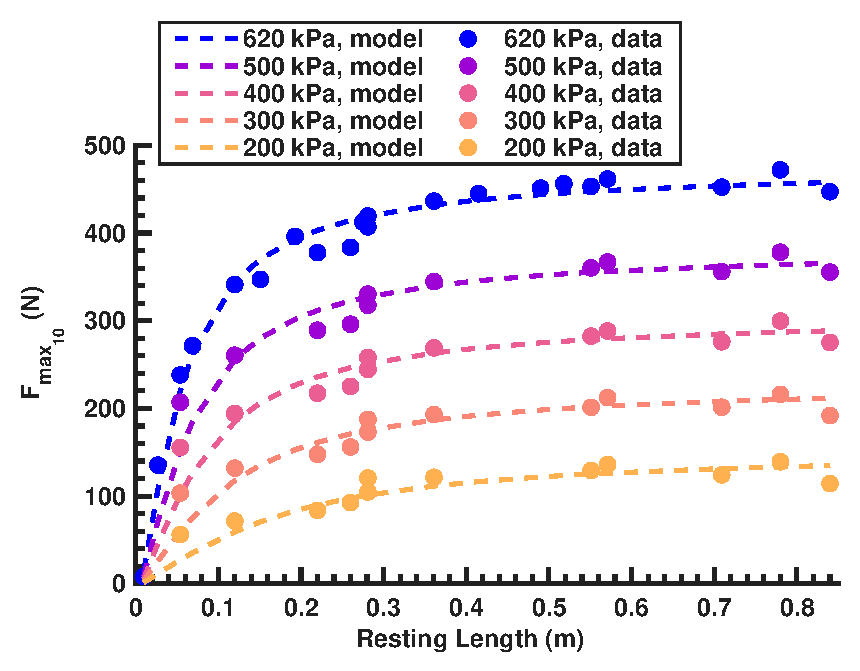
\includegraphics[width=13.3cm]{03a_MaxForce10_all.eps}}\\
\subfloat[\centering]{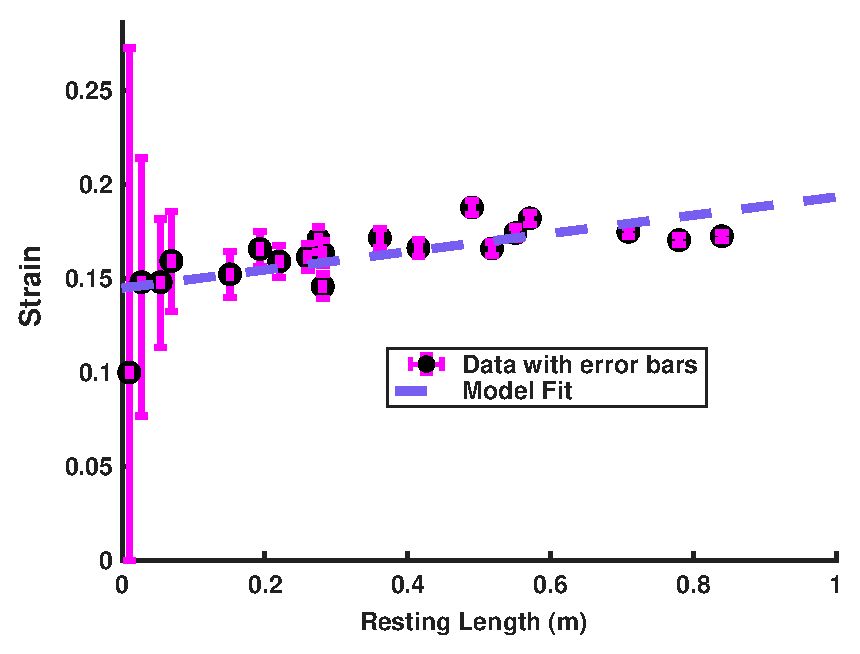
\includegraphics[width=13.8cm]{03b_kmax10.eps}}
%\end{adjustwidth}
\caption{\hl{Results} %MDPI: To avoid large blank spaces on the page, we moved Figure there. Please confirm.
 for finding the relationship between $F_{620}$, $l_{rest}$, $P_{620}$, and $\epsilon_{620_{10}}$. (\textbf{a}) Isoclines of the surface fit for $F_{620_{10}}(l_{rest},P_{620})$. (\textbf{b}) $\epsilon_{620_{10}}$ versus $l_{rest}$ at $P_{620}$. Although there is a general trend of longer resting lengths producing more contraction, no conclusive relationship between $\epsilon_{620}$ and $l_{rest}$ could be deduced from this experiment. The error bars show the effect of being $\pm$\qty{1}{\mm} in measuring $l_{rest}$ and $l_{620}$.}\label{fig:F-P_contraction}
\end{figure}





\begin{figure}[H]%[tbp]
%\begin{adjustwidth}{-\extralength}{0cm}
%\centering
\subfloat[\centering]{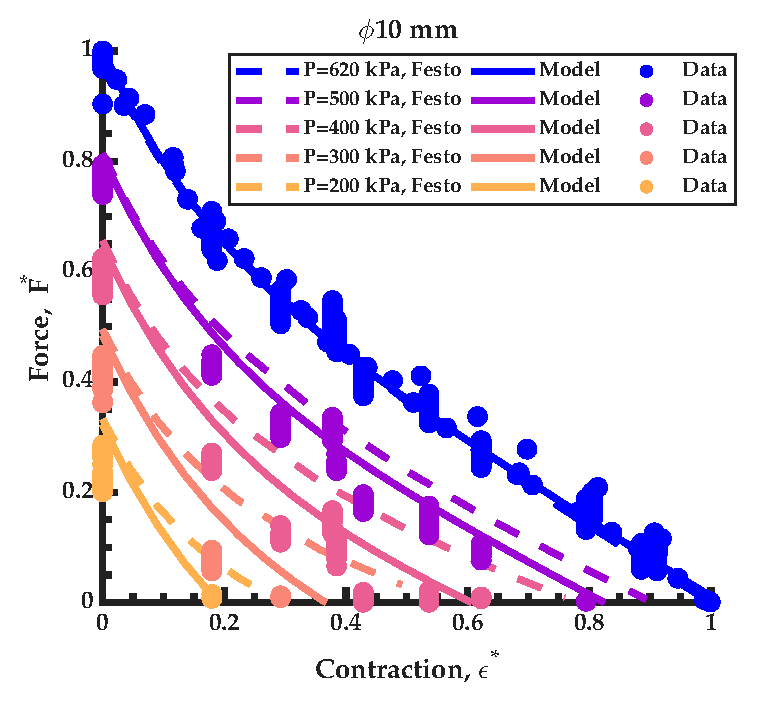
\includegraphics[width=10.88cm]{04a_FStar10.eps}}\\
\subfloat[\centering]{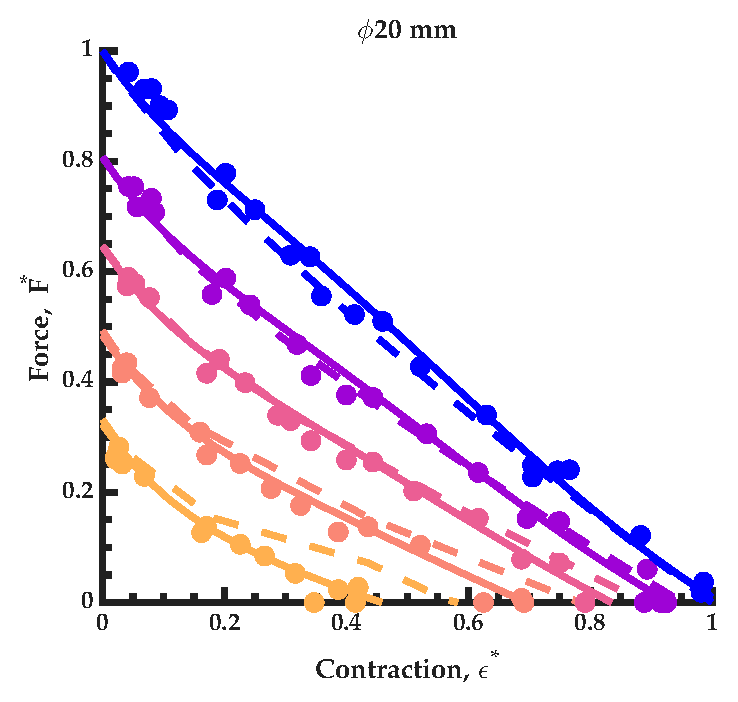
\includegraphics[width=10.88cm]{04b_FStar20.eps}}
%\end{adjustwidth}
\caption{Surface fit for $F^*(\epsilon^*,P^*)$. Solid lines are from our model. Dashed lines from Festo supplied data. In total, 537 data points were collected and used to fit the 3D surfaces (321 data points for $\phi$\qty{10}{\mm} BPAs and 216 data points for $\phi$\qty{20}{\mm} BPAs). In total, 80\% of these data were used for training, and 20\% were used for validation. For figure clarity, not all data is included and plotted circles represent collected data at $\pm\qty{10}{\kPa}$ of the stated pressure. (\textbf{a}) Fit data for $\phi$\qty{10}{\mm} Festo BPAs. (\textbf{b}) Fit data for $\phi$\qty{20}{\mm} Festo BPAs.}\label{fig:GenForceFit}
\end{figure}

We therefore derived our own equation for isometric force in the BPA as a function of pressure and contraction. Visual analysis of the experimental data shows an exponential relationship between $\epsilon^*$ and $F^*$, and a linear relationship between $P^*$ and $F$. We fit a surface to the data using Nonlinear Least Squares and a Least Absolute Residual robustness such that:
\begin{adjustwidth}{-\extralength}{0cm}
\begin{equation}
F^*(\epsilon^*,P^*)=
\begin{cases}
\begin{aligned}
c_0\cdot\bigl(\exp(-c_1 \cdot \epsilon^*)-1\bigr)
+ P^*\cdot\exp\!\bigl(-c_2(\epsilon^*)^{2}\bigr)
\end{aligned}
& \text{for } F^*>0\\[10pt]
0
& \text{for } F^*\le 0
\end{cases}\label{eq:exp}
\end{equation}
\end{adjustwidth}

For the $\phi$\qty{10}{\mm} BPAs, the result of the improved fit can be seen in Figure \ref{fig:GenForceFit}\hl{a}. The adjusted $\text{R}^2=0.9998$, a $\text{RMSE}=0.004537$, and a maximum absolute residual of $10.6\%$. Solving (\ref{eq:exp}) for the $\phi$\qty{20}{\mm} BPA, yields different coefficients, and results are seen in \mbox{Figure~\ref{fig:GenForceFit}\hl{b}.} Coefficient values and goodness-of-fit statistics are found in Table \ref{tab:Fstar}. 





\begin{table}[H]
\caption{\hl{Normalized} %MDPI: 1. We removed verticle lines in table, please confirm. 2. Please confirm if the left and right alignments necessary in table. 3. We put table not in landscape, please confirm.
 isometric BPA force equation (Equation~(\ref{eq:exp})) coefficient values and goodness-of-fit measures.}
\label{tab:Fstar}

\begin{adjustwidth}{-\extralength}{0cm}
%\centering %% If there is a figure in wide page, please release command \centering
\begin{tabularx}{\fulllength}{@{}lLLLllrllr@{}}
\toprule
\multirow{2.1}{*}{\textbf{BPA}} &
  \multirow{2.2}{*}{\textbf{Coefficient}} &
  \multirow{2.2}{*}{\textbf{CI (95\%)}} &
  \multicolumn{3}{c}{\textbf{Model}} &
  \multicolumn{3}{c}{\textbf{Validation}} \\ 
& & &
  \multicolumn{1}{l}{\textbf{Adj. $\text{R}^2$}} &
  \multicolumn{1}{l}{\textbf{RMSE}} &
  \textbf{Max. Error} &
  \multicolumn{1}{l}{\textbf{Adj. $\text{R}^2$}} &
  \multicolumn{1}{l}{\textbf{RMSE}} &
  \textbf{Max. Error} \\ \midrule
\multirow{3.8}{*}{$\phi$\qty{10}{\mm}} &
  $c_0 = 0.5682$ & (0.5584, 0.578) &
  \multicolumn{1}{l}{\multirow{3.8}{*}{0.9998}} &
  \multicolumn{1}{l}{\multirow{3.8}{*}{0.005118}} &
  \multirow{3.8}{*}{10.3\%} &
  \multicolumn{1}{l}{\multirow{3.8}{*}{0.9994}} &
  \multicolumn{1}{l}{\multirow{3.8}{*}{0.0245409}} &
  \multirow{3.8}{*}{10.6\%} \\ \cmidrule{2-3}
& $c_1 = 4.254$ & (4.126, 4.383) &
  \multicolumn{1}{l}{} & \multicolumn{1}{l}{} & &
  \multicolumn{1}{l}{} & \multicolumn{1}{l}{} & \\ \cmidrule{2-3}
& $c_2 = 0.5597$ & (0.5429, 0.5766) &
  \multicolumn{1}{l}{} & \multicolumn{1}{l}{} & &
  \multicolumn{1}{l}{} & \multicolumn{1}{l}{} & \\ \midrule
\multirow{3.8}{*}{$\phi$\qty{20}{\mm}} &
  $c_0 = 0.2579$ & (0.2401, 0.2756) &
  \multicolumn{1}{l}{\multirow{3.8}{*}{0.992}} &
  \multicolumn{1}{l}{\multirow{3.8}{*}{0.02294}} &
  \multirow{3.8}{*}{6.8\%} &
  \multicolumn{1}{l}{\multirow{3.8}{*}{0.9943}} &
  \multicolumn{1}{l}{\multirow{3.8}{*}{0.0231303}} &
  \multirow{3.8}{*}{5.7\%} \\ \cmidrule{2-3}
& $c_1 = 6.477$ & (5.558, 7.396) &
  \multicolumn{1}{l}{} & \multicolumn{1}{l}{} & &
  \multicolumn{1}{l}{} & \multicolumn{1}{l}{} & \\ \cmidrule{2-3}
& $c_2 = 1.321$ & (1.239, 1.403) &
\multicolumn{1}{l}{} & \multicolumn{1}{l}{} & &
\multicolumn{1}{l}{} & \multicolumn{1}{l}{} & \\ \bottomrule
\end{tabularx}
\end{adjustwidth}
\end{table}




%%%%%%%%%%%%%%%%%%%%%%%%%%%%%%%%%%%%%%%%%%
\section{Discussion}

\subsection{Effects of Resting Length}
We have developed new $F_{620}$ equations for \qtylist{10;20}{\mm} diameter Festo BPAs that capture the change in maximum force produced by the actuators at  \qty{620}{\kPa} as a function of their resting length. When examining Equation~(\ref{eq:Fmax10}) and measured data in Figure~\ref{fig:Fmax_fit}\hl{b}, it can be seen that as $l_{rest}$ goes to infinity, $F_{620_{10}}$ goes to \qty{470}{\N}. When the Festo tool \citep{lang_robert_musclesim_2005} was queried at $l_{rest}=\qty{1}{m}$ as an approximation of infinity, it predicts the $\phi$\qty{10}{\mm} BPA can produce $F=\qty{490}{\N}$ at $P_{620}$. This is within the 10\% variability that Festo states may occur in manufacturing tolerances. Similarly, the Festo data predict a $\phi$\qty{20}{\mm} BPA will produce $F=\qty{1570}{\N}$. Our results for Equation~(\ref{eq:Fmax20}) show that  $F_{620_{20}}$ goes to \qty{1460}{\N} as $l_{rest}$ approaches infinity. Although the difference is much larger, it is also with the \mbox{10\% manufacturing tolerance. }

Where our measured data differs significantly from the Festo model, is that as $l_{rest}$ goes to zero. For the measured data, as the length gets smaller, the force does as well, whereas the Festo tool predicts exponential force increase (see Figure~\ref{fig:Fmax_fit}). As a specific example, when specifying $l_{rest}=\qty{112}{\mm}$ for the \qtylist{10}{\mm} diameter BPAs, the Festo predicted $F_{620}$ is \qtylist{498.6}{\N}. However, using Equation~(\ref{eq:Fmax10}), $F_{620}$ is calculated to be \qtylist{335.3}{\N}. Actual force in the $l_{rest}=\qty{112}{\mm}$ was measured at \qtylist{350.9}{\N} Therefore, the error in predicted $F_{620}$ for the $\phi$\qty{10}{\mm} BPA is $4.5\%$ for our model and $42.1\%$ using the Festo tool. Researchers using BPA resting lengths under \qty{300}{\mm} should take note of these results.

\citet{festo_2026} (p.~12) states that force will be reduced by approximately 10\% for a minimum nominal length. In \citet{festo_2018} (p.~14) they say the force can deviate by 10\% based on factors such as: production variation, material variation, and deviation from nominal length ($l_{rest}$). \citet{festo_2013} (p.~13) notes that testing was done with BPAs that are ten times the uninflated diameter, and that theoretical force can increase by up to 10\%. In each datasheet, the characteristic curves appear to be the same. As demonstrated above, the \qty{100}{\mm} $\phi$\qty{10}{\mm} BPA should have much less force than what is shown in the curve. This is our experience and the reason for the testing. It is unclear why the \hl{MuscleSIM} %MDPI: Please state which version of the software was used.
 tool then predicts higher force as resting length decreases. It could be a reversed sign coefficient in their internal curve-fit model. We have shown here that as the nominal length goes to zero, so does force. 

The reason for BPA models predicting higher force than what is measured experimentally is a recurrent theme across many models: they do not account for the end effects of the pressure vessel where end effects dominate.	Nominally, the clamped ends fix the inner and outer diameter while allowing axial and radial displacement. In the isometric case, there is only radial displacement. The boundary conditions force steep gradients in stress and strain near the ends. Near the boundary conditions are where axial, radial, and circumferential strains deviate from analytic solutions to a cylindrical model. For a constant pressure, the end effect region appears to have the same length. Therefore, in shorter BPAs, the end effects dominate. The axial length scale of the boundary section is comparable to $l_{rest}$,  and the active force differs substantially from that of an assumed perfect cylinder.

Manufacturing variations seem to play an important factor in the behavior of these actuators. It remains to be seen how $\epsilon_{620}$ can be known a priori. We still suspect that it is a function of $l_{rest}$, but it might also be a function of other factors such as product batch number or UV light exposure \citep{festo_2026} (p.~15); \citep{festo_2018} (p.~6); \citep{festo_2013} \hl{(p.~13).} %MDPI: We revised ref. citation format and removed repeated content there, please confirm.
 We found there to be larger variations in the \qtylist{10}{\mm} BPAs than in the \qtylist{20}{\mm} BPAs. Modeling work of ideal McKibben actuators describe how the relationship between contraction and initial length is a function of the total number of twists and the angle of twist in the usable muscle area \citep{chou_measurement_1996}. It is unclear if there are variations in the angle and number of twists in the Festo BPAs due to manufacturing. Uncovering the relationship between $\epsilon_{620}$ and $l_{rest}$ for the Festo DMSP artificial muscles, if it exists in a meaningful way, will require additional controlled tests. 

Similarly, it is not clear how the maximum force might change with manufacturing variations. This was reasonably corrected for by normalizing the equations to each individual's maximum contraction, but more nuanced details might emerge with more data collection. Not knowing these relationships a priori means there is still a need for robots and other systems to go through an iterative design stage if it is discovered that the system does not produce the torque or have the RoM that the design team expects. However, the data and models provided here should enable for faster redesigns with fewer \mbox{additional measurements.}

\subsection{Nondimensionalization}

We have also introduced the concept of nondimensionalized isometric force that is a function of relative strain and relative pressure (Equation~(\ref{eq:exp})). This elegant equation has only three coefficients with low error (see Table~\ref{tab:Fstar}). In the work presented here, we introduce the relative pressure term, $P^*=P/P_{620}$. Our data show that by normalizing force, contraction, and pressure, we are able to create a simplified force equation as a function of contraction and pressure that scales well with initial actuator length, i.e.,
 \begin{equation}
   F(\epsilon^*,P^*,l_{rest}) = F^*(\epsilon^*,P^*) \cdot F_{620}(l_{rest}) \label{eq:force}
\end{equation}

For example, given $l_{rest}=\qty{54}{\mm}$ and $P=\qty{300}{\kPa}$, the measured force was \mbox{$F_{actual} = \qty{103}{\N}$.} Force prediction using only the Festo tool predicts the force to be \mbox{$F_{predict} = \qty{270}{\N}$.} This is $161\%$ greater than the measured force. Using Equations~(\ref{eq:Fmax10}) and~(\ref{eq:exp}) with Equation~(\ref{eq:force}) gives $F_{predict} = F^*(0, 0.48) \cdot F_{620}(0.054) = 0.49 \cdot \qty{230}{\N} = \qty{112}{\N}$. This is an error of $8\%$, which is much more accurate than using the Festo tool only.

The presented work is capable of predicting force output for 10 mm and 20 mm muscles with different initial muscle lengths, internal pressure, and contraction amount with minimal initial data collection. However, it remains to be seen if these relationships are maintained over the full lifecycle of the muscles. There are not yet any peer reviewed studies investigating the long-term behavior of these artificial muscles, though the Festo datasheet provides some indication of what can be expected \citep{festo_2026} (p.19). They report that the 40 mm BPA can complete 1 million cycles at \qty{6000}{\N} (maximum rated load), or 10 million cycles at \qty{4000}{\N}. The service life of the other size BPAs is not reported; however, it is mentioned that thermal stressing may reduce the lifespan and they should be inspected every 500,000 cycles for signs of aging \citep{festo_2018} (pp.~10--11). Future research should look at the behavior of these muscles over time.

In our work, $P_{620}=\qty{620}{\kPa}$ is the maximum supply pressure for our system, and other users of this actuator may use a different supply pressure. However, this supply pressure is not required, and normalizing by this value was chosen as a method for improving the optimization techniques by reducing the sensitivity of the term associated with pressure. This equation will work for any pressure supplies below \qty{620}{\kPa}. We also anticipate the equation will also work for pressures up to \qty{800}{\kPa} (the maximum rated pressure for Festo $\phi$\qty{10}{\mm} BPAs); however, we do not have the data to confirm this.

\subsection{Comparison with Other Published BPA Models}

The proposed model was compared with the formulations by \citet{sarosi_new_2012}, \citet{sarosi_10mm}, and \citet{martens_modeling_2017}, to evaluate their predictive performance across actuator sizes and operating conditions (see Table~\ref{tab:model_compare} and Figure~\ref{fig:ModelCompare}).
For the $\phi$\qty{20}{\mm} BPA, parameters from \cite{sarosi_new_2012} were used, corresponding to actuators with resting lengths of \qty{200}{\mm} and \qty{400}{\mm}. These were compared against the experimental data at $l_{rest}=\qty{300}{\mm}$ and $l_{rest}=\qty{450}{\mm}$, respectively. For the $\phi$\qty{10}{\mm} BPA with resting lengths of \qty{257}{\mm} and \qty{233}{\mm}, parameters from \cite{sarosi_10mm} were applied. In each case, the maximum contraction parameter ($k_{max}$) was determined numerically by solving $F(\qty{6.2}{\bar}, k_{max}) = 0$, ensuring consistency with the experimental maximum pressure condition.




\begin{table}[H]
\caption{\hl{Goodness-of-fit} %MDPI: 1. We removed verticle lines in table, please confirm. 2. Please add an explanation for the use of bold in the table footer. If the bold is unnecessary, please remove it in the table. 3. We put table not in landscape, please confirm. 4. We inserted it after where it is first mentioned in the text, please check and confirm.
 comparison for the Bolen, Sárosi, and Martens and Boblan models at different resting lengths (in mm) for \qty{10}{\mm} and \qty{20}{\mm} BPAs. RMSE and maximum error are reported in newtons, and FVU denotes the fraction of variance unexplained.}
\label{tab:model_compare}

\begin{adjustwidth}{-\extralength}{0cm}
%\centering %% If there is a figure in wide page, please release command \centering
\begin{tabularx}{\fulllength}{@{}lllllllllll@{}}
\toprule
\textbf{Diameter} &
  \textbf{Length} &
  \textbf{} &
  \textbf{Bolen} &
  \textbf{} &
  \textbf{} &
  \textbf{Sarosi} &
  \textbf{} &
  \textbf{} &
  \multicolumn{2}{l}{\textbf{Martens and Boblan}} \\ 
\textbf{} &
  \textbf{} &
  \textbf{RMSE} &
  \textbf{FVU} &
  \textbf{Max. Error} &
  \textbf{RMSE} &
  \textbf{FVU} &
  \textbf{Max Error} &
  \textbf{RMSE} &
  \textbf{FVU} &
  \textbf{Max. Error} \\ \midrule
\textbf{10 mm} & 257 & 22.9 & 0.0353 & 46.0  & 143.8 & 1.3903 & 235.8 & 73.8  & 0.3668 & 122.9  \\
\textbf{}      & 233 & 16.8 & 0.0187 & 30.3  & 132.7 & 1.1655 & 222.6 & 62.6  & 0.2590 & 101.2  \\ \midrule
\textbf{20 mm} & 300 & 35.6 & 0.0144 & 114.0 & 132.1 & 0.1992 & 313.4 & 72.8  & 0.0605 & 137.8  \\
\textbf{}      & 450 & 67.6 & 0.0258 & 166.6 & 177.7 & 0.1785 & 294.8 & 862.1 & 4.2022 & 1321.1 \\ \bottomrule
\end{tabularx}
\end{adjustwidth}
\end{table}

While the \citet{sarosi_new_2012} and \citet{sarosi_10mm} models capture general trends in force–contraction behavior, discrepancies were observed when applying parameters derived from different actuator lengths. In particular, the model tends to over-predict force at higher pressures and low amounts of contraction, suggesting sensitivity to geometric scaling effects not explicitly accounted for in the formulation.

The \citet{martens_modeling_2017} model  is derived from a geometric and material-based framework and provides a more physically grounded representation of actuator behavior. However, its accuracy depends strongly on precise geometric parameters, including braid angle, wall thickness, and fiber length. Small deviations in these parameters can lead to significant differences in predicted force, particularly at higher pressures.




\begin{figure}[H]%[tbp]
%\begin{adjustwidth}{-\extralength}{0cm}
%\centering
%\begin{center}
    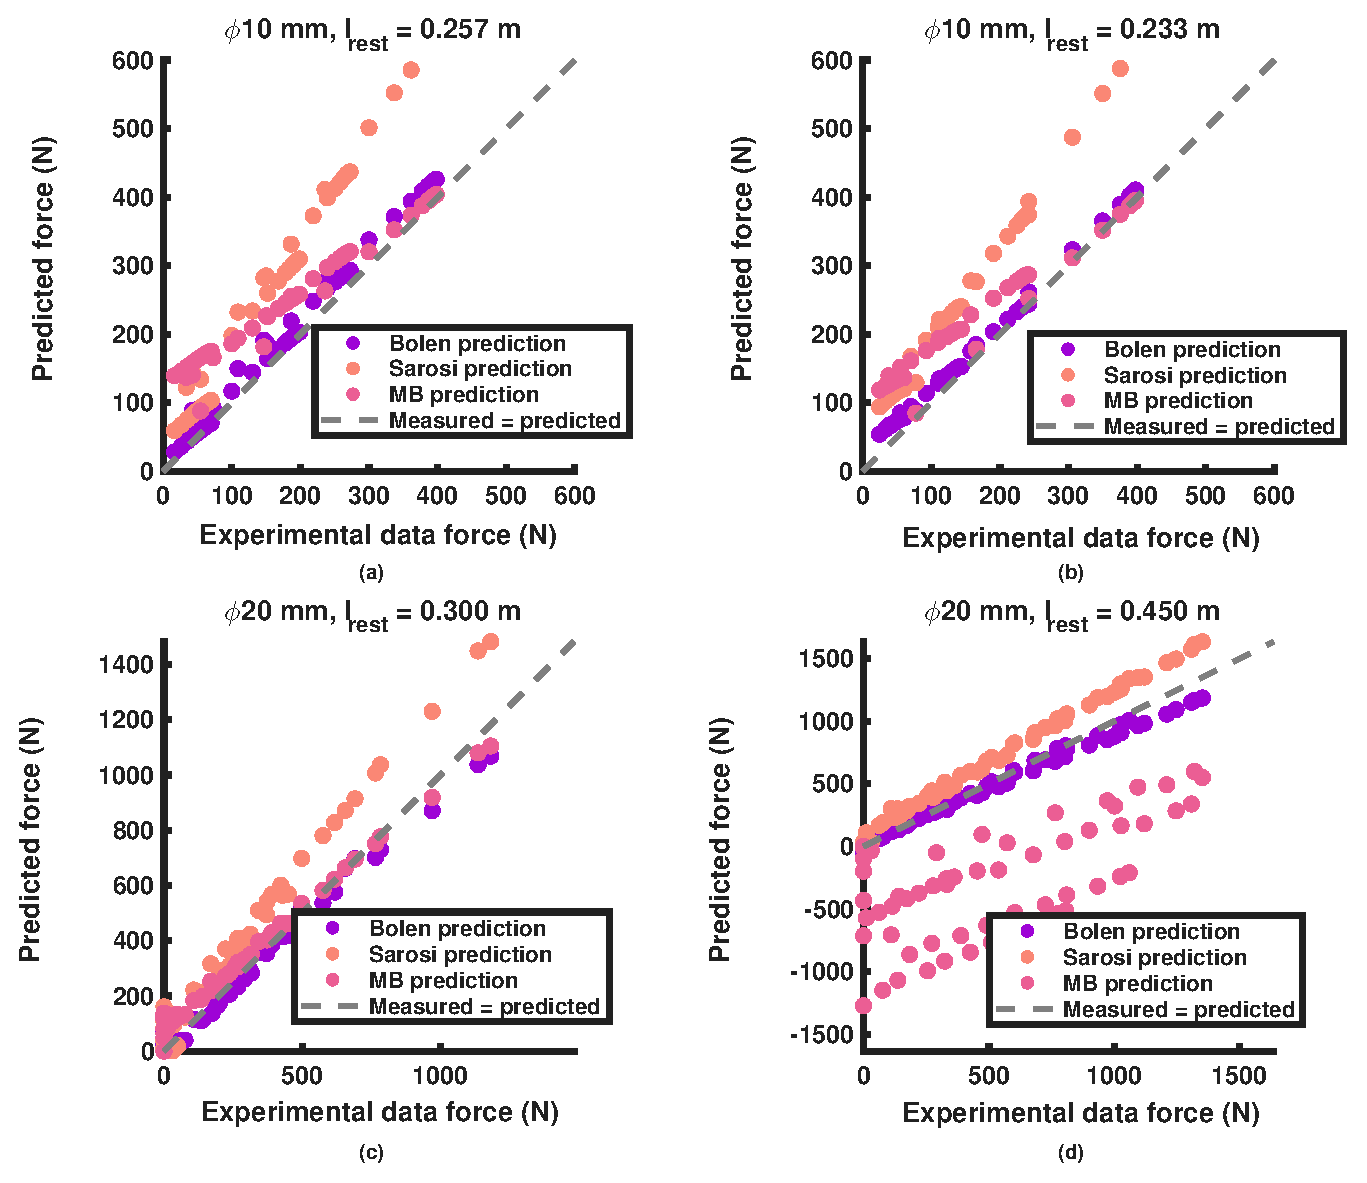
\includegraphics[width=.99\textwidth]{05_Comparison.eps}
%\end{center}
%\end{adjustwidth}
\caption{\hl{Comparison} %MDPI: 1. Please confirm whether the overlapping/incomplete content in this figure affects scientific understanding and if it does, please revise it. 2. We revised the hyphen in the figure into minus sign. Please confirm.
 between measured and predicted BPA force at varying amounts of contraction and pressure. A $y=x$ perfect fit line is added for reference. The BPAs compared are: (\textbf{a}) $\phi$\qty{10}{\mm}, $l_{rest}=\qty{0.257}{\mm}$, (\textbf{b}) $\phi$\qty{10}{\mm}, $l_{rest}=\qty{0.233}{\mm}$, (\textbf{c}) $\phi$\qty{20}{\mm}, $l_{rest}=\qty{0.300}{\mm}$, and (\textbf{d}) $\phi$\qty{20}{\mm}, $l_{rest}=\qty{0.450}{\mm}$.}\label{fig:ModelCompare}
\end{figure}






The Martens and Boblan model was first evaluated at the same pressure–contraction points as in their experimental data \citep{martens_modeling_2017} \hl{(Tables A1 and  A2),} %MDPI: There is no Tables A1 and  A2 of the text, please correct the citation or confirm if it belongs to ref. [18].
 indicating that it reproduces the general published force map shape but is sensitive to the assumed initial geometry. %MDPI EE: Please check intended meaning has been retained
  Examining their $\phi$\qty{20}{\mm} BPA, for example, using the explicitly stated $l_{rest}=\qty{300}{\mm}$ and initial diameter $D_{0}=\qty{20}{\mm}$ significantly under-predicted the results compared to using the implied $l_{rest}=\qty{296}{\mm}$ (\citep{martens_modeling_2017} \hl{(}%MDPI: Please confirm if () out of Tabel A1 is necessary.
\hl{Table A1}%MDPI: There is no Table A1 of the text, please correct the citation or confirm if it belongs to ref. [18].
)) and $D_{0}+H_{0}=\qty{21.8}{\mm}$, where $H_{0}=\qty{1.8}{\mm}$ is the material thickness. The diameter adjustment can be implied \mbox{from \citep{chou_measurement_1996}.} This adjusted diameter was also included for the $\phi$\qty{10}{\mm} BPA to give a better fit. As can be seen in Figure~\ref{fig:ModelCompare} and Table~\ref{tab:model_compare}, the highest accuracy is observed when $\phi$\qty{20}{\mm} and $l_{rest}=\qty{300}{\mm}$, which is at or very near their experimental measurements. For the $\phi$\qty{10}{\mm} BPAs the accuracy decreases even though their experimentally measured $l_{rest}=\qty{250}{\mm}$ is close to our $l_{rest}=\qty{257}{\mm}$ and $l_{rest}=\qty{233}{\mm}$. The largest error occurs at $\phi$\qty{20}{\mm} and $l_{rest}=\qty{450}{\mm}$ and the model starts to predict negative force. We have calculated that the $F_{PE}\cdot\frac{dD}{DL}$ term becomes very large compared to the others \citep{martens_modeling_2017} (p.~5). This suggests that the model is sensitive to geometric parameter selection and interpretation, particularly with respect to initial length and diameter definitions.

In comparison, the present normalized model demonstrates improved consistency across actuator lengths by incorporating experimentally derived scaling through $F_{620}$ and $\epsilon_{620}$. This normalization reduces sensitivity to geometric variation and enables a unified representation of actuator behavior, while maintaining predictive accuracy over the tested range of pressures and contractions.

\subsection{Implications for Real-Time Control and Simulation}

Although pneumatic muscle actuators exhibit hysteresis, thermodynamic effects, and other dynamic behavior, accurate and high-performance controller designs can still be achieved using a static force map approach when the underlying static force model is accurate. Martens and Boblan explicitly note that BPA dynamics are often dominated by the air dynamics inside the actuator and the mass flow behavior of the valve, such that precise modeling of the static force characteristic remains crucial for torque control \mbox{accuracy \citep{martens_modeling_2017}.} This view is consistent with more recent BPA control work, including a sensor-less torque control interface for BPA-driven joints \citep{martens_framework_2018}, stable force/position/stiffness control of antagonistic pneumatic-muscle joints \citep{ugurlu2019stable, hunt_development_2017}, and sensor-less angle stiffness control of antagonistic BPA systems \citep{shinSensorlessAngleStiffness2022}. 

In this context, the present model is well suited for real-time use because it reduces the static isometric force prediction to a low-order normalized surface, $F^*(\epsilon^*,P^*)$, scaled by the resting-length-dependent term $F_{620}(l_{rest})$. This structure is computationally inexpensive to evaluate online and is also suitable for lookup-table implementation. While the present work does not model the full actuator--valve dynamics, it provides the static force relationship needed as a feedforward or inner-model component in real-time torque control, simulation, and preliminary design workflows. It is anticipated that improved real-time control for high-speed and high-precision systems will benefit more from improved modeling of airflow dynamics than dynamics involving actuator hysteresis, damping, and other dynamic behavior.


\subsection{Biomimetic Artificial Muscle Analogy}

BPA artificial muscles are often said to be analogous to biological muscles because they have force--length curves and can produce force only in tension. This analogy is worth closer inspection. For example, the describes the passive force–length curve has been described as an exponential function arising from connective tissue elements, while the active force–length relationship is typically modeled as a bell-shaped curve reflecting actin–myosin overlap \citep{winters1990}. These formulations emphasize that muscle force generation is governed by nonlinear geometric and material interactions rather than simple linear elasticity.
McKibben-type pneumatic artificial muscles (of which Festo is an example) exhibit analogous nonlinear behavior, though arising from fundamentally different physical mechanisms. As shown by Chou and Hannaford, the force–length relationship of McKibben actuators is derived from geometric constraints imposed by the braided shell, leading to a nonlinear dependence of force on actuator length through the braid angle \cite{chou_measurement_1996}. In their formulation, actuator force is proportional to pressure and a nonlinear geometric term $(3\cos^2\theta - 1)$, which governs both the maximum contraction limit and the curvature of the force–length relationship. The work presented here demonstrates that this nonlinear curve can be well approximated by an exponential as well.

However, there are some distinct differences between how these artificial muscles behave when compared to biological muscles.
For example, the biological muscle optimum fiber length $l_{OFL}$ is not equivalent to $l_{rest}$ in the muscles. The maximum active force that the artificial muscles can produce is at the resting length, also the maximum length, of the artificial muscles. In contrast, the maximum active force a biological muscle length can produce is somewhere in the middle of the total contractile length of the muscle. 

Furthermore, biological muscles can adapt the optimal operating length through structural remodeling (e.g., sarcomere addition or tendon compliance) while BPAs have a fixed geometric configuration. This allows biological systems to self-optimize for the particular tasks the animal is subjected to. In order to re-optimize a robot for new tasks, new actuators would have to be swapped into the system. This distinction highlights a key limitation of BPAs in biomimetic applications, while also reinforcing the importance of accurate nonlinear modeling for control and design.


\section{Conclusions}

%This study developed improved equations for predicting isometric force in Festo \qtylist{10;20}{\mm} BPAs. The results show that maximum isometric force at \qty{620}{\kPa}, $F_{620}$, depends on resting length, and that normalized force can be represented accurately as a function of relative strain and relative pressure. Together, the $F_{620}(l_{rest})$ fits and the nondimensional force surface $F^*(\epsilon^*,P^*)$ provide a practical static force model for actuator selection, simulation, and controller design.

The analysis in this study has created novel equations for calculating force in Festo \qtylist{10;20}{\mm} diameter BPAs. This study has elucidated the relationship between maximum BPA force at 620 kPa $F_{620}$ as a function of resting length $l_{rest}$ (\mbox{Equations~(\ref{eq:Fmax10}) and~(\ref{eq:Fmax20}),} Table~\ref{tab:Fmax}). We have also created more accurate equations for the nondimensionalized force in a BPA as a function of relative strain $\epsilon^*$ and relative pressure $P^*$, (Equation~(\ref{eq:exp}) and \mbox{Table~\ref{tab:Fstar}}). Taken together, the $F_{620}(l_{rest})$ fits and the nondimensional force surface $F^*(\epsilon^*,P^*)$ provide a practical way to predict isometric BPA force across resting lengths using a small number of measurements. In a design workflow, these equations make it easier to select actuator diameter and resting length, and to evaluate whether a proposed routing can meet force and range-of-motion requirements before committing to a full prototype. As a result, BPA-driven mechanisms (e.g., joints in biomimetic legs or manipulators) can be developed with fewer design iterations and with realistic expectations of force output at short \mbox{resting lengths.}



%%%%%%%%%%%%%%%%%%%%%%%%%%%%%%%%%%%%%%%%%%
\vspace{6pt} 

%%%%%%%%%%%%%%%%%%%%%%%%%%%%%%%%%%%%%%%%%%
%% optional
%\supplementary{The following supporting information can be downloaded at:  \linksupplementary{s1}, Figure S1: title; Table S1: title; Video S1: title.}


% Only used for preprtints:
% \supplementary{The following supporting information can be downloaded at the website of this paper posted on \href{https://www.preprints.org/}{Preprints.org}.}

%%%%%%%%%%%%%%%%%%%%%%%%%%%%%%%%%%%%%%%%%%
\authorcontributions{Conceptualization, B.B. and A.H..; Methodology, B.B., A.H., M.E. and L.P.; Software, B.B., M.E. and L.P.; Validation, B.B. and A.H.; Formal Analysis, B.B.; Investigation, B.B., M.E. and L.P.; Resources, B.B. and A.H.; Data Curation, B.B. and L.P.; Writing---Original Draft Preparation, B.B.; Writing---Review and Editing, B.B., M.E., L.P. and A.H.; Visualization, B.B. and A.H.; Supervision, B.B. and A.H.; Project Administration, B.B. and A.H.; Funding Acquisition, A.H. All authors have read and agreed to the published version of the manuscript.}

\funding{\hl{Research} %MDPI: Information regarding the funder and the funding number should be provided. Please check the accuracy of funding data and any other information carefully.
 for this article was funded by the Department of Mechanical and Materials Engineering at Portland State University, the National Science Foundation (NSF) grant for NeuroNex: Communication, Coordination, and Control in Systems (C3NS) 2015317 and NSF grant 1943483. }

\dataavailability{The data sets are available from the authors upon reasonable request.} 

\acknowledgments{\hl{The} %MDPI: Please ensure that all individuals included in this section have consented to the acknowledgement.
 authors would like to thank Jasmine Bradley for her help reworking the figures in the \hl{results section.} %MDPI: Please confirm if it should be Section 4.
 As a visual designer, her contributions improved the aesthetic quality of the images and ensured data accessibility for people with color blindness. Furthermore, the authors would like to express their gratitude towards Cody Scharzenberger for all his assistance in proof-reading and editing the manuscript.}

\conflictsofinterest{The authors declare no conflicts of interest. The funders had no role in the design of the study; in the collection, analyses, or interpretation of data; in the writing of the manuscript; or in the decision to publish the results.} 

%%%%%%%%%%%%%%%%%%%%%%%%%%%%%%%%%%%%%%%%%%
%% Optional

\abbreviations{Abbreviations}{
The following abbreviations are used in this manuscript:
\\

\vspace{-6pt}\noindent 
\begin{tabular}{@{}ll}
BPA & Braided Pneumatic Actuator\\
\end{tabular}
}


%%%%%%%%%%%%%%%%%%%%%%%%%%%%%%%%%%%%%%%%%%
%\isPreprints{}{% This command is only used for ``preprints''.
\begin{adjustwidth}{-\extralength}{0cm}
%} % If the paper is ``preprints'', please uncomment this parenthesis.
%\printendnotes[custom] % Un-comment to print a list of endnotes

\reftitle{References}

% Please provide the correct journal abbreviation (e.g. according to the “List of Title Word Abbreviations” http://www.issn.org/services/online-services/access-to-the-ltwa/).
% Citations and References in Supplementary files are permitted provided that they also appear in the reference list here. 

%=====================================
% References, variant A: external bibliography
%=====================================
\begin{thebibliography}{999}

\bibitem[Andrews(1985)]{andrews_general_1985}
Andrews, J.G.
\newblock A {General} {Method} for {Determining} the {Functional} {Role} of a
  {Muscle}.
\newblock {\em J. Biomech. Eng.} {\bf 1985}, {\em
  107},~348--353.
\newblock {\url{https://doi.org/10.1115/1.3138568}}.

\bibitem[Millard et~al.(2013)Millard, Uchida, Seth, and
  Delp]{millard_flexing_2013}
Millard, M.; Uchida, T.; Seth, A.; Delp, S.L.
\newblock Flexing {Computational} {Muscle}: {Modeling} and {Simulation} of
  {Musculotendon} {Dynamics}.
\newblock {\em J. Biomech. Eng.} {\bf 2013}, {\em
  135},~021005.
\newblock {\url{https://doi.org/10.1115/1.4023390}}.

\bibitem[Arnold et~al.(2010)Arnold, Ward, Lieber, and Delp]{arnold_model_2010}
Arnold, E.M.; Ward, S.R.; Lieber, R.L.; Delp, S.L.
\newblock A {Model} of the {Lower} {Limb} for {Analysis} of {Human} {Movement}.
\newblock {\em Ann. Biomed. Eng.} {\bf 2010}, {\em 38},~269--279.
\newblock {\url{https://doi.org/10.1007/s10439-009-9852-5}}.
\newpage
\bibitem[Asano et~al.(2017)Asano, Okada, and Inaba]{asano_design_2017}
Asano, Y.; Okada, K.; Inaba, M.
\newblock Design principles of a human mimetic humanoid: {Humanoid} platform to
  study human intelligence and internal body system.
\newblock {\em Sci. Robot.} {\bf 2017}, {\em 2}, eaaq0899.
\newblock {\url{https://doi.org/10.1126/scirobotics.aaq0899}}.

\bibitem[Asano et~al.(2019)Asano, Okada, and Inaba]{asano_musculoskeletal_2019}
Asano, Y.; Okada, K.; Inaba, M.
\newblock Musculoskeletal design, control, and application of human mimetic
  humanoid {Kenshiro}.
\newblock {\em Bioinspir. Biomim.} {\bf 2019}, {\em 14},~036011.
\newblock {\url{https://doi.org/10.1088/1748-3190/ab03fc}}.

\bibitem[Hitzmann et~al.(2018)Hitzmann, Masuda, Ikemoto, and
  Hosoda]{hitzmann_anthropomorphic_2018}
Hitzmann, A.; Masuda, H.; Ikemoto, S.; Hosoda, K.
\newblock Anthropomorphic musculoskeletal 10 degrees-of-freedom robot arm
  driven by pneumatic artificial muscles.
\newblock {\em Adv. Robot.} {\bf 2018}, {\em 32},~865--878.
\newblock {\url{https://doi.org/10.1080/01691864.2018.1494040}}.

\bibitem[Liu et~al.(2018)Liu, Rosendo, Ikemoto, Shimizu, and
  Hosoda]{liu_robotic_2018}
Liu, X.; Rosendo, A.; Ikemoto, S.; Shimizu, M.; Hosoda, K.
\newblock Robotic investigation on effect of stretch reflex and crossed
  inhibitory response on bipedal hopping.
\newblock {\em J. R. Soc. Interface} {\bf 2018}, {\em 15}, \hl{20180024.} %MDPI: We removed extra content, please confirm the revisions in all refs.
  {\url{https://doi.org/10.1098/rsif.2018.0024}}.

\bibitem[Chen et~al.(2019)Chen, Zhong, Kang, and Qiao]{chen_realizing_2019}
Chen, J.; Zhong, S.; Kang, E.; Qiao, H.
\newblock Realizing human-like manipulation with a musculoskeletal system and
  biologically inspired control scheme.
\newblock {\em Neurocomputing} {\bf 2019}, {\em 339},~116--129.
\newblock {\url{https://doi.org/10.1016/j.neucom.2018.12.069}}.

\bibitem[Ijspeert(2020)]{ijspeert_amphibious_2020}
Ijspeert, A.J.
\newblock Amphibious and {Sprawling} {Locomotion}: {From} {Biology} to
  {Robotics} and {Back}.
\newblock {\em Annu. Rev. Control. Robot. Auton. Syst.} {\bf
  2020}, {\em 3},~173--193.
\newblock {\url{https://doi.org/10.1146/annurev-control-091919-095731}}.

\bibitem[He and Gao(2020)]{he_mechanism_2020}
He, J.; Gao, F.
\newblock Mechanism, {Actuation}, {Perception}, and {Control} of {Highly}
  {Dynamic} {Multilegged} {Robots}: {A} {Review}.
\newblock {\em Chin. J. Mech. Eng.} {\bf 2020}, {\em
  33},~79.
\newblock {\url{https://doi.org/10.1186/s10033-020-00485-9}}.

\bibitem[Liang et~al.(2020)Liang, Liu, Wang, Qian, Ren, and
  Ren]{liang_comparative_2020}
Liang, W.; Liu, H.; Wang, K.; Qian, Z.; Ren, L.; Ren, L.
\newblock Comparative study of robotic artificial actuators and biological
  muscle.
\newblock {\em Adv. Mech. Eng.} {\bf 2020}, {\em
  12},~1687814020933409.
\newblock {\url{https://doi.org/10.1177/1687814020933409}}.

\bibitem[Veale and Xie(2016)]{veale_towards_2016}
Veale, A.J.; Xie, S.Q.
\newblock Towards compliant and wearable robotic orthoses: {A} review of
  current and emerging actuator technologies.
\newblock {\em Med. Eng. Phys.} {\bf 2016}, {\em 38},~317--325.
\newblock {\url{https://doi.org/10.1016/j.medengphy.2016.01.010}}.

\bibitem[Suzumori and Faudzi(2018)]{suzumori_trends_2018}
Suzumori, K.; Faudzi, A.A.
\newblock Trends in hydraulic actuators and components in legged and tough
  robots: A review.
\newblock {\em Adv. Robot.} {\bf 2018}, {\em 32},~458--476.
\newblock {\url{https://doi.org/10.1080/01691864.2018.1455606}}.

\bibitem[Madden et~al.(2004)Madden, Vandesteeg, Anquetil, Madden, Takshi,
  Pytel, Lafontaine, Wieringa, and Hunter]{madden_artificial_2004}
Madden, J.; Vandesteeg, N.; Anquetil, P.; Madden, P.; Takshi, A.; Pytel, R.;
  Lafontaine, S.; Wieringa, P.; Hunter, I.
\newblock Artificial muscle technology: Physical principles and naval
  prospects.
\newblock {\em IEEE J. Ocean. Eng.} {\bf 2004}, {\em
  29},~706--728.
\newblock {\url{https://doi.org/10.1109/JOE.2004.833135}}.

\bibitem[Hunt et~al.(2017)Hunt, Graber-Tilton, and Quinn]{hunt_modeling_2017}
Hunt, A.; Graber-Tilton, A.; Quinn, R.
\newblock Modeling length effects of braided pneumatic actuators.
\newblock In \emph{\hl{ASME 2017 International Design Engineering Technical Conferences and Computers and Information in Engineering Conference.} %MDPI: We completed the title, please confirm.
 Volume {5A}: 41st {Mechanisms} and {Robotics}
  {Conference}, \hl{Cleveland, OH}%MDPI: Please confirm 
};  \hl{American Society of Mechanical Engineers: New York, NY, USA,} %MDPI: We added the name of the publisher and their location. Please confirm. Same as below.
 2017; Volume 58172, p. V05AT08A008.
\newblock {\url{https://doi.org/10.1115/detc2017-67458}}.

\bibitem[Aschenbeck et~al.(2006)Aschenbeck, Kern, Bachmann, and
  Quinn]{aschenbeck_design_2006}
Aschenbeck, K.; Kern, N.; Bachmann, R.; Quinn, R.
\newblock Design of a {Quadruped} {Robot} {Driven} by {Air} {Muscles}.
\newblock In \emph{The {First} {IEEE}/{RAS}-{EMBS} {International}
  {Conference} on {Biomedical} {Robotics} and {Biomechatronics}, 2006. {BioRob}
  2006};  \hl{IEEE: Piscataway, NJ, USA,} 2006; \mbox{pp. 875--880.}
\newblock {\url{https://doi.org/10.1109/BIOROB.2006.1639201}}.

\bibitem[Sárosi et~al.(2017)Sárosi, Piteľ, Tóthová, Hošovský, and
  Bíró]{sarosi_comparative_2017}
Sárosi, J.; Piteľ, J.; Tóthová, M.; Hošovský, A.; Bíró, I.
\newblock {\hl{COMPARATIVE} %MDPI: Please confirm if all uppercase letters of title are necessary of the ref.
} {SURVEY} {OF} {VARIOUS} {STATIC} {AND} {DYNAMIC}
  {MODELS} {OF} {PNEUMATIC} {ARTIFICIAL} {MUSCLES}.
\newblock {\em Trans. Can. Soc. Mech. Eng.}
  {\bf 2017}, {\em 41},~825--844.
\newblock {\url{https://doi.org/10.1139/tcsme-2017-514}}.

\bibitem[Martens and Boblan(2017)]{martens_modeling_2017}
Martens, M.; Boblan, I.
\newblock Modeling the {Static} {Force} of a {Festo} {Pneumatic} {Muscle}
  {Actuator}: {A} {New} {Approach} and a {Comparison} to {Existing} {Models}.
\newblock {\em Actuators} {\bf 2017}, {\em 6},~33.
\newblock {\url{https://doi.org/10.3390/act6040033}}.

\bibitem[{Festo AG \& Co. KG}(2026)]{festo_2026}
{Festo AG \& Co. KG}.
\newblock Fluidic Muscle DMSP.
\newblock [Product Datasheet].\hl{ 2026.} %MDPI: We moved the year there, please confirm.
 Available online:
  \url{https://www.festo.com/media/catalog/202851_documentation.pdf} (accessed
  on 26 March 2026).

\bibitem[Lang(2005)]{lang_robert_musclesim_2005}
Lang, R.
\newblock \emph{\hl{MuscleSIM}%MDPI: Please provide version of software.
}, \hl{Dept. TK-ES, Festo AG \& Co. KG.:} %MDPI: Please provide full name of publisher if possible.
  \hl{Esslingen am Neckar, Germany,} %MDPI: We added the location of publisher, please confirm. Same as below.
  2005;
\newblock \hl{[Software]; not publicly available.} %MDPI: Please confirm if the content is necessary.


\bibitem[{Festo AG \& Co. KG}(2018)]{festo_2018}
{Festo AG \& Co. KG}.
\newblock \hl{Fluidic Muscle DMSP/MAS. } %MDPI: The content is same as ref. 22, please confirm Refs. 21 and 22 are duplicated. If they are, please remove duplicated references and rearrange all the references so that they appear in numerical order. Please ensure that there are no duplicated references. if not, please confirm if the content are correct.
\newblock [Product Datasheet]. \hl{2018.} %MDPI: We moved the year there, please confirm.
 Available online:
  \url{https://www.festo.com/net/en_us/SupportPortal/Files/732773/DMSP_MAS_2018-01f_8081496g1.pdf}
  (accessed on 26 March 2026).

\bibitem[{Festo AG \& Co. KG}(2013)]{festo_2013}
{Festo AG \& Co. KG}.
\newblock \hl{Fluidic Muscle DMSP/MAS.}
\newblock [Product Datasheet]. \hl{2013.} %MDPI: We moved the year there, please confirm.
 Available online:
  \url{https://ftp.festo.com/Public/PNEUMATIC/SOFTWARE_SERVICE/Documentation/2015/EN/DMSP-MAS_EN.PDF}
  (accessed on 26 March 2026).

\bibitem[Chou and Hannaford(1996)]{chou_measurement_1996}
Chou, C.P.; Hannaford, B.
\newblock Measurement and modeling of {McKibben} pneumatic artificial muscles.
\newblock {\em IEEE Trans. Robot. Autom.} {\bf 1996}, {\em
  12},~90--102.
\newblock {\url{https://doi.org/10.1109/70.481753}}.

\bibitem[Sárosi(2012)]{sarosi_new_2012}
Sárosi, J.
\newblock New approximation algorithm for the force of fluidic muscles.
\newblock In\emph{\hl{2012 7th IEEE International Symposium on Applied Computational Intelligence and Informatics (SACI)}%MDPI: We revised the title, please confirm.
}; IEEE: \hl{Piscataway, NJ, USA,}
   2012; pp. 229--233.

\bibitem[Sárosi and Fabulya(2012)]{sarosi_10mm}
Sárosi, J.; Fabulya, Z.
\newblock Mathematical analysis of the function approximation for the force
  generated by pneumatic artificial muscle.
\newblock {\em Sci. Bull. Politeh. Univ. Timiș. Trans. Mech.} {\bf 2012}, {\em 57},~59--64.

\bibitem[Martens et~al.(2018)Martens, Seel, Zawatzki, and
  Boblan]{martens_framework_2018}
Martens, M.; Seel, T.; Zawatzki, J.; Boblan, I.
\newblock A {Novel} {Framework} for a {Systematic} {Integration} of
  {Pneumatic}-{Muscle}-{Actuator}-{Driven} {Joints} into {Robotic} {Systems}
  {via} a {Torque} {Control} {Interface}.
\newblock {\em Actuators} {\bf 2018}, {\em 7},~82.
\newblock {\url{https://doi.org/10.3390/act7040082}}.

\bibitem[Ugurlu et~al.(2019)Ugurlu, Forni, Dallali, Caldwell, and
  Tsagarakis]{ugurlu2019stable}
Ugurlu, B.; Forni, P.E.; Dallali, H.; Caldwell, D.G.; Tsagarakis, N.G.
\newblock Stable {Control} of {Force}, {Position}, and {Stiffness} for a
  {Pneumatic} {Muscle} {Actuator} {Joint}.
\newblock {\em Trans. Ind. Inform.} {\bf 2019}, {\em
  15}, \hl{1240--1251.} %MDPI: 1. We cannot access the link to this doi. Please check and provide an available doi. 2. We are sorry but we could not find the ref. information.  Please check and  confirm if the ref. correct.
\newblock {\url{https://doi.org/10.1109/TII.2018.2849330}}.

\bibitem[Hunt et~al.(2017)Hunt, Szczecinski, and Quinn]{hunt_development_2017}
Hunt, A.; Szczecinski, N.; Quinn, R.
\newblock Development and {Training} of a {Neural} {Controller} for {Hind}
  {Leg} {Walking} in a {Dog} {Robot}.
\newblock {\em Front. Neurorobot.} {\bf 2017}, {\em 11}, 18.
\newblock {\url{https://doi.org/10.3389/fnbot.2017.00018}}.

\bibitem[Shin and Kogiso(2022)]{shinSensorlessAngleStiffness2022}
Shin, T.; Kogiso, K.
\newblock Sensorless angle and stiffness control of antagonistic {PAM} actuator
  using reference set.
\newblock {\em Adv. Robot.} {\bf 2022}, {\em 36},~423--437.
\newblock {\url{https://doi.org/10.1080/01691864.2022.2046502}}.

\bibitem[Winters(1990)]{winters1990}
Winters, J.M.
\newblock Hill-{Based} {Muscle} {Models}: {A} {Systems} {Engineering}
  {Perspective}. In {\em Multiple {Muscle} {Systems}: {Biomechanics} and
  {Movement} {Organization}};  Winters, J.M., Woo, S.L.Y., Eds.;
  Springer: New York, NY,  USA, 1990; pp. 63--93.
\newblock {\url{https://doi.org/10.1007/978-1-4613-9030-5_5}}.

\end{thebibliography}


% If authors have biography, please use the format below
%\section*{Short Biography of Authors}
%\bio
%{\raisebox{-0.35cm}{\includegraphics[width=3.5cm,height=5.3cm,clip,keepaspectratio]{Definitions/author1.pdf}}}
%{\textbf{Firstname Lastname} Biography of first author}
%
%\bio
%{\raisebox{-0.35cm}{\includegraphics[width=3.5cm,height=5.3cm,clip,keepaspectratio]{Definitions/author2.jpg}}}
%{\textbf{Firstname Lastname} Biography of second author}

% For the MDPI journals use author-date citation, please follow the formatting guidelines on http://www.mdpi.com/authors/references
% To cite two works by the same author: \citeauthor{ref-journal-1a} (\citeyear{ref-journal-1a}, \citeyear{ref-journal-1b}). This produces: Whittaker (1967, 1975)
% To cite two works by the same author with specific pages: \citeauthor{ref-journal-3a} (\citeyear{ref-journal-3a}, p. 328; \citeyear{ref-journal-3b}, p.475). This produces: Wong (1999, p. 328; 2000, p. 475)

%%%%%%%%%%%%%%%%%%%%%%%%%%%%%%%%%%%%%%%%%%
%% for journal Sci
%\reviewreports{\\
%Reviewer 1 comments and authors’ response\\
%Reviewer 2 comments and authors’ response\\
%Reviewer 3 comments and authors’ response
%}
%%%%%%%%%%%%%%%%%%%%%%%%%%%%%%%%%%%%%%%%%%
\PublishersNote{}
%\isPreprints{}{% This command is only used for ``preprints''.
\end{adjustwidth}
%} % If the paper is ``preprints'', please uncomment this parenthesis.
\end{document}

